\documentclass[]{article}

\usepackage{amsmath}
\usepackage{amssymb}
\usepackage{empheq}
\usepackage{graphicx}
\usepackage{float}
\usepackage{subcaption}
\usepackage{hyperref}
\usepackage{doi}

%opening
\title{Derivation of the BPM equations}
\author{Mike Machielsen}

\begin{document}	
	\maketitle
	
	
	\section{Intro}
	Photonic integrated circuits (PICs) have applications in many areas. However, to properly design them we need to simulate them accurately. There are many ways to do that, one of them being the beam propagation method (BPM). It cuts some corners in the physics, but it is very fast, typically orders of magnitude faster than EME or FDTD. Which makes it a useful tool to rapidly comb through the parameter space. The more rigorous EME/FDTD solvers can then be used to do the final optimization.\\	
	
	These notes describe how one such BPM is implemented here. It is not the goal of these notes to exhaustively describe BPM, for that see Ref. \cite{Lifante_2015}. The derivation in these notes follows along the lines of the book, but differs in some notation and choice of coordinates. %also there are some critical typos in the book I think..., so that is reason enough to rederive it and confirm.
	
	\section{Coordinate system}
	The typical coordinate system is shown in Fig. \ref{fig:coordinates}. The propagation direction is the $z$ direction, the $x$ direction is normal to the PIC, and $y$ is tangent to the PIC. This I will refer to as ``classical coordinates'', since it is used most often in BPM literature.\\
	
	I will define another right-handed Cartesian coordinate system, called ``nazca coordinates''. This is convenient for integration with PIC layout software as we usually view the PIC from above and call the horizontal direction $x$ and the vertical $y$. Both of these lie in the plane of the PIC, so the $z$ direction is normal to the PIC. Also by convention the propagation direction is usually from left to right, when viewing from above, so that would be the $x$ direction. In short, we make the following substitution:
	\begin{subequations}
		\begin{align}
			x_\text{nazca} &= z_\text{classical}\, ,\\
			y_\text{nazca} &= -y_\text{classical}\, , \\
			z_\text{nazca} &= x_\text{classical}\, .
		\end{align}
	\end{subequations}
	

	\begin{figure}[t!]
		\centering
		\begin{subfigure}[t]{0.5\textwidth}
			\centering
			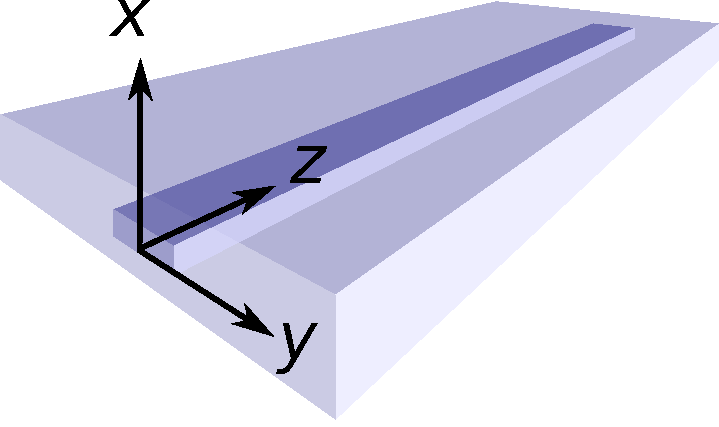
\includegraphics[height=3cm]{coordinates_classic.pdf}
			\caption{Classical coordinates.}
		\end{subfigure}%
		~ 
		\begin{subfigure}[t]{0.5\textwidth}
			\centering
			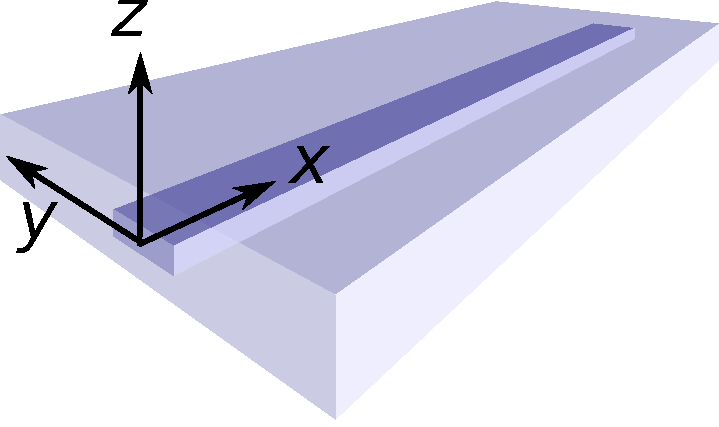
\includegraphics[height=3cm]{coordinates_nazca.pdf}
			\caption{Nazca/Klayout coordinates.}
		\end{subfigure}
		\caption{Coordinate systems used in this project. The purple box in the middle represents the structure of interest. See also Fig. 2.1 of \cite{Lifante_2015}.\label{fig:coordinates}}
	\end{figure}
	
	The coordinate change does not modify the final equations. All we do is shift the names by one: $x \to y; y \to z; z \to x$. Since the notation of ``up'' is arbitrary anyway, we can just rotate the PIC around the new $x$ axis, or rotate the coordinate system in the opposite direction, and we have the nazca coordinates.\\
	
	Unless specified otherwise, nazca coordinates will be used from now on.
	
	
	\section{Beam propagation method}
	Let us start from the very basis, Maxwell's equations.
	\subsection{Maxwell's equations}
	Maxwell's equations in macroscopic form are as follows:
	\begin{subequations}
		\begin{align}
			\nabla \cdot \textbf{D} &= \rho_f \, , \\
			\nabla \cdot \textbf{B} &= 0 \, ,\\
			\nabla \times \textbf{E} &= -\frac{\partial \textbf{B}}{\partial t}\, ,\\
			\nabla \times \textbf{H} &= \textbf{J}_f + \frac{\partial \textbf{D}}{\partial t} \, ,
		\end{align}
		\label{Maxwell}
	\end{subequations}
	where $\textbf{D}$ is the electric displacement, $\textbf{H}$ the magnetizing field, $\textbf{E}$ the electric field, and $\textbf{B}$ the magnetic field. $\rho_f$ is the free charge density, and $\textbf{J}_f$ the free current density.\\
	
	We will now make an assumption on the constitutive relation, let the medium be linear, isotropic and local. So, the auxiliary fields are
	\begin{subequations}
		\begin{align}
			\textbf{D} &= \varepsilon \textbf{E}\, ,\\
			\textbf{B} &= \mu \textbf{H} \, .
		\end{align}
	\end{subequations}
	Typically materials in the world of integrated photonics are non-magnetic, so $\mu = \mu_0$. But material properties will depend on the position (inhomogeneous), and on the frequency of the light (dispersive). We will also assume that $\varepsilon$ is constant in time.\\
	
	Free currents follow Ohm's law (to good approximation):
	\begin{equation}
		\textbf{J}_f = \sigma \textbf{E} \, ,
	\end{equation}
	with $\sigma$ the material's conductivity. PICs have very low conductivity, so free currents are usually neglected. From charge conservation we can also derive that if $\textbf{J}_f \approx \textbf{0}$, the free charge is constant in time, so negligible too (zero initial conditions).\\
	
	In summary we have so far:
		\begin{subequations}
		\begin{align}
			\nabla \cdot \left( \varepsilon \textbf{E}\right)  &= 0\, , \\
			\nabla \cdot \textbf{H} &= 0 \, ,\\
			\nabla \times \textbf{E} &= -\mu_0 \frac{\partial \textbf{H}}{\partial t}\, ,\label{test1}\\			
			\nabla \times \textbf{H} &= \varepsilon \frac{\partial \textbf{E}}{\partial t} \, , 	\label{test2}		
		\end{align}
		\label{Maxwell2}
	\end{subequations}
	By combining Eq. \eqref{test1}, \eqref{test2} we obtain the double curl equation:
	\begin{equation}
		\nabla \times \left( \nabla \times \textbf{E}\right)  +\mu_0 \varepsilon \partial_t^2 \textbf{E} = \textbf{0}\,.
		\label{double_curl_time}
	\end{equation}	
	You can also obtain a double curl equation for the $\textbf{H}$ field, but most BPM solvers use the $\textbf{E}$ field. There is no strong preference for either formulation, but it makes sense to solve for the field we care about the most, the $\textbf{E}$ field. Hence that is what we do here.\\
	
	The vector Laplacian is defined as $\nabla^2 \textbf{A} := \nabla(\nabla\cdot \textbf{A})-\nabla \times \nabla \times \textbf{A}$, so we can write Eq. \eqref{double_curl_time} as:
	\begin{equation}
		\nabla^2 \textbf{E} -  \nabla(\nabla\cdot \textbf{E}) -\mu_0 \varepsilon \partial_t^2 \textbf{E} = \textbf{0}\, .
	\end{equation}
	
	In the frequency domain $\partial_t \to i\omega$. Also we will define $k_0 := \omega/c$, and the refractive index as $n:=\sqrt{\varepsilon/\varepsilon_0}$, so we get:
	\begin{equation}
		\nabla^2 \textbf{E} -  \nabla(\nabla\cdot \textbf{E}) +n^2k_0^2 \textbf{E} = \textbf{0}\, .
	\end{equation}
	From Gauss's law we have $\varepsilon \nabla\cdot \textbf{E} = - \frac{1}{\varepsilon}\nabla \varepsilon \cdot \textbf{E}$, so we can write:
	\begin{equation}
		\nabla^2 \textbf{E} +  \nabla\left( \frac{\nabla(n^2)}{n^2}\cdot \textbf{E}\right)  +n^2k_0^2 \textbf{E} = \textbf{0}\, .
		\label{Laplacian_eq}
	\end{equation}
	
	Eq. \eqref{Laplacian_eq} is actually three equations:
	\begin{subequations}
		\begin{align}
			\nabla^2 E_x + \frac{\partial}{\partial x}\left(\frac{1}{n^2}\frac{\partial n^2}{\partial x} E_x+\frac{1}{n^2}\frac{\partial n^2}{\partial y} E_y+\frac{1}{n^2}\frac{\partial n^2}{\partial z} E_z \right)+n^2 k_0^2 E_x = 0\, ,\\ 
			\nabla^2 E_y + \frac{\partial}{\partial y}\left(\frac{1}{n^2}\frac{\partial n^2}{\partial x} E_x+\frac{1}{n^2}\frac{\partial n^2}{\partial y} E_y+\frac{1}{n^2}\frac{\partial n^2}{\partial z} E_z \right)+n^2 k_0^2 E_y = 0\, ,\\
			\nabla^2 E_z + \frac{\partial}{\partial z}\left(\frac{1}{n^2}\frac{\partial n^2}{\partial x} E_x+\frac{1}{n^2}\frac{\partial n^2}{\partial y} E_y+\frac{1}{n^2}\frac{\partial n^2}{\partial z} E_z \right)+n^2 k_0^2 E_z = 0\, .
		\end{align}
	\end{subequations}
	
	We will now limit ourselves to \textbf{slowly varying} structures in the propagation direction $x$, so we may neglect $\partial_x n^2$. So for the two transverse components we have:
	\begin{subequations}
		\begin{align}
			\nabla^2 E_y + \frac{\partial}{\partial y}\left(\frac{1}{n^2}\frac{\partial n^2}{\partial y} E_y+\frac{1}{n^2}\frac{\partial n^2}{\partial z} E_z \right)+n^2 k_0^2 E_y = 0\, ,\\ 
			\nabla^2 E_z + \frac{\partial}{\partial z}\left(\frac{1}{n^2}\frac{\partial n^2}{\partial y} E_y+\frac{1}{n^2}\frac{\partial n^2}{\partial z} E_z \right)+n^2 k_0^2 E_z = 0\, .
		\end{align}
		\label{main_eqs}
	\end{subequations}
	
	
	\subsection{BPM equations}
	We may define the envelope function $\Psi$ in the following way, which is still without additional approximations:
	\begin{subequations}
		\begin{align}
			E_y(x,y,z) = \Psi_y(x,y,z) e^{-ik_0 n_0 x}\, ,\\
			E_z(x,y,z) = \Psi_z(x,y,z) e^{-ik_0 n_0 x}\, ,
		\end{align}
		\label{envelope_split}
	\end{subequations}
	where $n_0$ is a yet to be chosen ``reference index''\footnote{This is another weakness of BPM. You have to choose $n_0$. Typically we choose this equal to the effective index. But what do you do when this varies in the propagation direction, or what if you have multiple modes with a different effective index? You can choose $n_0$ equal to the average of those, but the approximation of Eq. \eqref{paraxial_approx} will not be accurate for every mode and every $x$ position.}. 
	Since the propagation is mainly along $x$ direction, and the structures are varying slowly in that direction, the envelope function will vary slowly in $x$ direction, compared to the rapidly oscillating phase term. More explicitly,
	we have:
	\begin{equation}
		\left|\frac{\partial^2 \Psi_y}{\partial x^2} \right| \ll n_0 k_0 \left| \frac{\partial \Psi_y}{\partial x} \right|\, ,
		\label{paraxial_approx}
	\end{equation}
	and the same for $\Psi_z$. This is called the Paraxial approximation. This is somewhat crude, but also very powerful, all the second order derivatives in $x$ drop out. We are left with only a first order derivative in $x$, and given an input field at $x=0$ (analogous to an initial condition), we can march along the $x$ direction and calculate the field at any $x>0$. The steps $\Delta x$ can be on the wavelength scale $1/k_0$ or even larger, since the phase part is eliminated.\\
	
	Plugging Eq. \eqref{envelope_split} into Eq. \eqref{main_eqs} and applying the Paraxial approximation yields:
	\begin{subequations}
		\begin{align}
			2i k_0 n_0 \frac{\partial \Psi_y}{\partial x} &= \frac{\partial^2\Psi_y}{\partial y^2}+\frac{\partial^2\Psi_y}{\partial z^2}+\frac{\partial}{\partial y}\left(\frac{1}{n^2}\frac{\partial n^2}{\partial y} \Psi_y+\frac{1}{n^2}\frac{\partial n^2}{\partial z} \Psi_z \right)+k_0^2(n^2-n_0^2)\Psi_y \, ,\\
			2i k_0 n_0 \frac{\partial \Psi_z}{\partial x} &= \frac{\partial^2\Psi_z}{\partial y^2}+\frac{\partial^2\Psi_z}{\partial z^2}+\frac{\partial}{\partial z}\left(\frac{1}{n^2}\frac{\partial n^2}{\partial y} \Psi_y+\frac{1}{n^2}\frac{\partial n^2}{\partial z} \Psi_z \right)+k_0^2(n^2-n_0^2)\Psi_z  \, .
		\end{align}
	\end{subequations}
	
	This can be refactored as:
	\begin{subequations}
		\begin{align}
			2i k_0 n_0 \frac{\partial \Psi_y}{\partial x} &= P_{yy} \Psi_y+P_{yz} \Psi_z \, ,\\
			2i k_0 n_0 \frac{\partial \Psi_z}{\partial x} &= P_{zz} \Psi_z+P_{zy} \Psi_y \, .
		\end{align}
		\label{bpm_eq1}
	\end{subequations}
	with the following definitions:
	\begin{subequations}
		\begin{align}
			P_{yy} f &:= \frac{\partial}{\partial y}\left(\frac{1}{n^2}\frac{\partial (n^2 f)}{\partial y}  \right)+\frac{\partial^2 f}{\partial z^2}+k_0^2(n^2-n_0^2)f\, , \\
			P_{yz} f &:= \frac{\partial}{\partial y}\left(\frac{1}{n^2}\frac{\partial (n^2 f)}{\partial z}  \right) - \frac{\partial^2 f}{\partial y \partial z}\, ,\\
			P_{zy} f &:= \frac{\partial}{\partial z}\left(\frac{1}{n^2}\frac{\partial (n^2 f)}{\partial y}  \right) - \frac{\partial^2 f}{\partial y \partial z}\, ,\\
			P_{zz} f &:= \frac{\partial}{\partial z}\left(\frac{1}{n^2}\frac{\partial (n^2 f)}{\partial z}  \right)+\frac{\partial^2 f}{\partial y^2}+k_0^2(n^2-n_0^2)f\, .\\
		\end{align}
	\end{subequations}
	The operator has been rewritten in such a way that the derivative applies to $n^2 \Psi_y$ and $n^2 \Psi_z$ as a whole. This is convenient, because the normal component of $\textbf{E}$ may be discontinuous at a dielectric interface. However, $\textbf{D}$ is not. Likewise, $\Psi$ may be discontinuous, but $n^2 \Psi$ is not.
	
	\subsection{Semi-Vectorial formulation}
	In this case we neglect index variations in one transverse direction\footnote{In addition to the $z$ direction, because we already neglected $\partial_z n^2$.}, so that the two equations \eqref{bpm_eq1} decouple (the cross terms disappear). 
		
	\subsection{Scalar formulation}
	In this case we neglect index variations in two transverse directions. This reduces Eq. \eqref{bpm_eq1} down to just one equation:
	\begin{equation}
		2i k_0 n_0 \frac{\partial u}{\partial x} = \frac{\partial^2u}{\partial y^2}+\frac{\partial^2u}{\partial z^2}+k_0^2(n^2-n_0^2)u \, ,\\
		\label{scalar_eq}
	\end{equation}
	with $u$ the scalar envelope. The distinction between TE and TM modes is lost in this representation. Note the similarity between Eq. \eqref{scalar_eq} and the heat equation or diffusion equation. The time derivative is replaced by a derivative with respect to $x$. And an initial condition is replaced by an input profile. Instead of marching in time we advance the solution along the $x$ direction.
	
	
	\subsection{Numerical implementation}	
	We will try to find an approximate solution to Eq. \eqref{scalar_eq} using finite differences. We can calculate $u(x+\Delta x,y, z)$ from $u(x,y,z)$ with many different methods. For instance, 4th order explicit Runge-Kutta is very popular; it is easy to implement and accurate. Because it is an \textit{explicit} method, we only need to do a matrix-vector multiply to update the field, so it also requires little RAM. However, in order for the method to be stable, the maximal step size for explicit methods is limited to \cite{Chung_Dagli_1991}:
	\begin{equation}
		\Delta x < 2 k_0 n_0 \left[\frac{4}{\min (\Delta y)^2} +\frac{4}{\min(\Delta z)^2}+k_0^2\left| n_{\text{max}}^2-n_0^2\right|  \right] ^{-1}\, .
	\end{equation}	
	For example, for a typical grid size of $\Delta y= \Delta z $ = 10 nm, we have $\Delta x < 0.1$ nm\footnote{Depending on precise material settings, just using typical values here.}. This is very unfortunate because one big advantage of BPM is that we do not need to resolve the sub-wavelength scale in propagation direction $x$. But with an explicit method we have to, not because of the truncation error, but because of stability of the scheme.\\
	
	\textit{Implicit} schemes on the other hand are usually unconditionally stable, which means that the step size along $x$ can be arbitrarily large\footnote{Do not conflate stability with accuracy, just because it is stable does not mean the solution is accurate.}. The downside of implicit methods is that we have to solve a linear system (of the type $Ax=b$) at every iteration. This is far more expensive than a single explicit iteration, but it is still worth it because $\Delta x$ can be orders of magnitude larger. Most BPM solvers implement the Crank-Nicolson scheme. It is second order accurate, and the matrix to invert is tri-diagonal. This means we can apply the Thomas algorithm which has a time complexity of $O(N)$, where $N$ is the number of grid points in the $yz$ mesh.\\
	
	Following along Section 3.2.2 of Ref. \cite{Lifante_2015}, we define the operator $G$:
	\begin{subequations}
		\begin{align}
			G &:= G_y+G_z \, ,\\
			G_y &:=\frac{\partial^2}{\partial y^2}+\frac{1}{2}k_0^2(n^2-n_0^2)\, ,\\
			G_z &:=\frac{\partial^2}{\partial z^2}+\frac{1}{2}k_0^2(n^2-n_0^2)\, .\\
		\end{align}		
	\end{subequations}
	This splitting is important later on, so that we can apply the alternating direction implicit (ADI) method. Eq. \eqref{scalar_eq} can be written as:
	\begin{equation}
		2i k_0 n_0 \frac{\partial u}{\partial x} = G u = G_y u + G_z u\, .
		\label{G_operator_on_u}
	\end{equation}
	We will use a rectangular mesh to grid $y,z$:
	\begin{subequations}
		\begin{align}
			y_p = y_{\text{min}}+\Delta y\cdot p \quad, p = 0,1,...,P-1\, ,\\
			z_q = z_{\text{min}}+\Delta z\cdot q \quad, q = 0,1,...,Q-1\, .
		\end{align}
	\end{subequations}
	The value of $u$ on these grid points we will indicate as $u_{p,q}^r$. Where the superscript $r$ indicates the step along the propagation direction. These values can be stored in a vector:
	\begin{equation}
		u^r := \begin{pmatrix}
			u_{0,0}\\
			u_{0,1}\\
			u_{0,2}\\
			...\\
			u_{1,0}\\
			u_{1,1}\\
			u_{1,2}\\
			...\\
			u_{P-1,Q-3}\\
			u_{P-1,Q-2}\\
			u_{P-1,Q-1}\\
			\end{pmatrix}
			\label{uvector}
	\end{equation}
	So we get\footnote{Points on the boundary of the domain are set by the BCs, and do not need to be updated, see section \ref{BC_section}. So Eq. \eqref{scalar_eq_discretized} is only applied to the inside of the grid.}:
	\begin{equation}
		2ik_0 n_0 \frac{u^{r+1}-r^r}{\Delta x} = (1-\alpha)\left( G_y u^r+G_z u^r\right) +\alpha\left( G_y u^{r+1}+G_z u^{r+1}\right)\, .
		\label{scalar_eq_discretized}
	\end{equation}
	This is a weighted sum between the forward and backward Euler methods, with $\alpha\in[0,1]$ is the scheme parameter. If $\alpha=0$ we have the forward Euler method, with $\alpha=1$ we have the backward Euler method, and with $\alpha=1/2$ we have the classical Crank-Nicolson method. For stability we require $\alpha \ge 0.5$. See \cite{Lifante_2015} for a lengthy discussion on the best choice for $\alpha$, in short, we typically choose a value slightly over 0.5. Note, the operators $G_y, G_z$ in Eq. \eqref{scalar_eq_discretized} are discretized as well using finite differences.
	\begin{equation}
		\frac{\partial^2 u}{\partial y^2} \to \frac{u_{p+1,q}-2u_{p,q}+u_{p-1,q}}{\Delta y^2}\, .
		\label{double_derivative}
	\end{equation}
	
	Rearranging Eq. \eqref{scalar_eq_discretized} gives:
	\begin{equation}
		\left(1+\frac{i\alpha \Delta x}{2k_0 n_0}(G_y+G_z) \right) u^{r+1} = \left(1-\frac{i(1-\alpha) \Delta x}{2k_0 n_0}(G_y+G_z) \right) u^r \, .
	\end{equation}
	The operator on the left hand side (LHS) is a matrix with five non-zero diagonal bands. In order to factor it into two tri-diagonal matrices we add a negligible extra term on both the LFS and RHS:
	
	\begin{multline*}
		\left(1+\frac{i\alpha \Delta x}{2k_0 n_0}(G_y+G_z) + \left(\frac{i\alpha \Delta x}{2k_0 n_0} \right) ^2 G_y G_z \right) u^{r+1} =\\
		 \left(1-\frac{i(1-\alpha) \Delta x}{2k_0 n_0}(G_y+G_z) +\left( \frac{i(1-\alpha) \Delta x}{2k_0 n_0}\right)^2 G_y G_z \right) u^r \, ,
	\end{multline*}
	which we can factor to get:
	\begin{multline}
		\left(1+\frac{i\alpha \Delta x}{2k_0 n_0}G_y \right)\left(1+\frac{i\alpha \Delta x}{2k_0 n_0}G_z \right) u^{r+1} = \\
		\left(1-\frac{i(1-\alpha) \Delta x}{2k_0 n_0}G_y \right)\left(1-\frac{i(1-\alpha) \Delta x}{2k_0 n_0}G_z \right) u^r \, .
		\label{ADI_setup}
	\end{multline}
	
	Note: up to here we followed along the lines of the book\cite{Lifante_2015}. But I don't understand what Lifante does next. In Eq. (3.78) there is the $G_z$ operator, not the $G_y$ operator. Surely you would ``peel away'' one operator by multiplying with the inverse from the left on both sides, which means we invert the operator with $G_y$ first, then $G_z$... I am not sure that is correct.\\
	
	So we will now follow the procedure of Masoudi, chapter 6.2.1 \cite{masoudi1995parallel}, since this is what I would have done too. First we define the following vectors:
	\begin{subequations}
		\begin{align}
			V^r &:= \left(1+\frac{i\alpha \Delta x}{2k_0 n_0}G_z \right) u^r\, ,\\
			W^r &:= \left(1-\frac{i(1-\alpha) \Delta x}{2k_0 n_0}G_y \right)\left(1-\frac{i(1-\alpha) \Delta x}{2k_0 n_0}G_z \right) u^r \, .
		\end{align}
	\end{subequations}
	This is just a definition, so no further approximations are made. Eq. \eqref{ADI_setup} can be written as:
	\begin{equation}
		\left(1+\frac{i\alpha \Delta x}{2k_0 n_0}G_y \right) V^{r+1} = W^r\, .
	\end{equation}
	The right hand side is readily computed, it only needs the old field values, which are known. The vector $V^{r+1}$ is yet to be determined, so the first step is to invert the operator on the left. Since it contains only the derivative in one direction this is a tri-diagonal matrix\footnote{Strictly speaking it is not tri-diagonal. The bands are not near the diagonal, they are $Q$ bands away because of the formatting of the solution vector. The next grid neighbor in $y$ direction is $Q$ rows down in Eq. \eqref{uvector}. This is no problem though, you could just reformat it into $Q$ independent problems with each a tri-diagonal matrix. Solve it, then format back. Note, this reformatting is just a way of explaining the math, in the actual implementation this can be skipped for more efficient memory usage.}, which we can rapidly solve with the Thomas algorithm. Now that we have $V^{r+1}$, the last step is to solve for $u^{r+1}$ in yet another tri-diagonal problem:
	\begin{equation}
		\left(1+\frac{i\alpha \Delta x}{2k_0 n_0}G_z \right) u^{r+1} = V^{r+1}\, .
	\end{equation}
	
	\subsection{Boundary conditions}
	\label{BC_section}	
	Note, the perfectly matched layer (PML) is not itself a boundary condition (BC), it is a layer that sits \textit{inside} of your modeling domain. You still need to specify an actual BC on the edge of the domain. For this we will go with the simplest possible one, homogeneous Dirichlet BCs, i.e. $u=0$. This will not result in any significant reflection because the light will need to pass through the PML twice before entering back into the region of interest. The PML uses a parabolic conductivity profile.\\
	
	We will use these BCs and PML in the two transverse directions. Since Eq. \eqref{scalar_eq} is a one-way wave model we only need one BC in the propagation direction: the input field. No BC is needed, nor can it be specified, at the final $x$ location where the simulation stops.\\
	
	The derivation of PML is rather lengthy, but the end result is the following substitution in Eq. \eqref{scalar_eq}:
	\begin{subequations}
		\begin{align}
			\frac{\partial^2 u}{\partial y^2} \to \eta \frac{\partial}{\partial y}\left(  \eta \frac{\partial u}{\partial y}\right) \, ,\\
			\frac{\partial^2 u}{\partial z^2} \to \xi \frac{\partial}{\partial z}\left(  \xi \frac{\partial u}{\partial z}\right) \, .
		\end{align}
	\end{subequations}
	Where $\eta$ is defined as:
	\begin{equation}
		\eta := \left(1-\frac{i\sigma(y)}{\varepsilon_0 \omega n^2} \right)^{-1}\, .
	\end{equation}
	The conductivity profile is:
	\begin{equation}
		\sigma(y):= \begin{cases}
			\sigma_{\text{max}}\left( \frac{y-(\delta-L/2)}{\delta}\right)^2 \, &, y <-L/2+\delta\\
			0&, -L/2+\delta \le y \le L/2 - \delta\\
			\sigma_{\text{max}}\left( \frac{y-(L/2-\delta)}{\delta}\right)^2 \, &, y > L/2 - \delta
		\end{cases}
	\end{equation}
	and $\delta$ is the PML thickness and $\sigma_{\text{max}}$ the PML strength. In the $z$ direction the same procedure is applied with $\xi$ (not shown here). In the corners of the domain two PMLs will overlap, but this is not a problem. Notice that the equations are not modified anywhere, except inside the PML. The second derivative is now discretized as follows:
	\begin{multline}
		\eta \frac{\partial}{\partial y}\left(  \eta \frac{\partial u}{\partial y}\right)  \to\\
		\frac{\eta_{p,q}}{2\Delta y^2}\left[(\eta_{p,q}+\eta_{p+1,q})u_{p+1,q} -(\eta_{p+1,q}+2\eta_{p,q}+\eta_{p-1,q})u_{p,q}+(\eta_{p,q}+\eta_{p-1,q})u_{p-1,q}\right] 
	\end{multline}
	
	
	Clarification about the BCs: You can choose to set $u$ to zero on the actual wall of the domain. Or set $u=0$ outside the domain, but let the value on the boundary vary freely. The distinction seems irrelevant, since we are interested in open domains anyway. However, the latter approach may be easier to implement, as you do not need to skip over the first and last row+column of the grid. You can just loop over all matrix entries, then where-ever the derivative requires outside information you just use zero. However, this will also require outside information for the index $n$. This is dangerous because the index outside the domain is invisible to the end-user. So we will go with the first option, setting $u=0$ on the actual wall.

	
	\bibliographystyle{ieeetr}
	\bibliography{bibliography}
	
\end{document}
